% Chapter 2

\chapter{Introduction} % Main chapter title

\label{Chapter2} % For referencing the chapter elsewhere, use \ref{Chapter1} 

\section{Background and Context}

Precise knowledge about the biomechanical characterization of soft tissues has received attention
in medical research, e.g., medical image analysis and visualization.
For many years, the obtained medical diagnosis have come from assumptions of experts or 
accumulated experience. This information, although proven to be useful, has its limitations 
when computed-assisted systems like, medical diagnosis, therapy, and training, rely on 
more quantifiable data \cite{Kauer2002}. To gather this data, it is important to gain access
to the tissues and perform in-vivo testing experiments. For organs, this procedure is nearly 
impossible to achieve, due to the involvement of an invasive procedure, and the lack of constant
and reproducible external and internal factors. \\ 

One of the complications associated with the extraction of the organ is that some material 
properties may change despite examination of the same organ. Their biomechanical properties 
depend on other factors, such as changes in blood pressure, changes in material properties 
over time, symptoms from diseases, etc. Furthermore, another encountered issue is the lack 
of replication, due to the use of different individuals organs, which includes more external
 factors to add to the equation. Moreover, given a tissue sample, it is difficult to 
 characterize the organ's material properly due to its anisotropy property. The material 
 properties change, resulting in an inaccurate result.
%not only due to the lack of a tissue sample, but also because the time-dependent material properties. 
\\

\section{Problem Statement}
In the situation where the soft material's data can be gather in a constant, fast and reliable
process, the data enables the system to predict the behavior of soft tissues and give pre-operative
 calculations. This shows that material models represent a vital part for medical research, 
 specially for the use of computational models, as their help to increase the accuracy of the 
 simulation and its applications in other systems.\\

In soft materials analyses, a nonlinear situation is mostly encountered, for which a finite 
element method becomes a common approach. The application of the finite element method
 facilitates the analysis of complex structures with complex material behavior, and aids in 
 solving of continuum mechanical problems. Nevertheless, in order to simulate a material with 
 this complexity also requires complex algorithms with high computational costs. \\

 \section{Objective and Scope of the Study} 
One of the goals of this study to identify the key parameters of soft materials, and their 
influence in the development of a material model. With key parameters an attempt to 
 approximate a complex material will be done, and this simplified material model will be 
 validated for its future applications in medical research.\\
 
 With the application of experiment testing, and the finite element method it is possible 
 to identify some key material parameters through an inverse finite element method approach. With this 
 method a framework can be established and the results of computational model can be matched 
 to the experimental data, and afterwards be validated with other validation point data.

 \section{cgt}
 %wechsel
 %Due to the complexity of the polymer microstructure, the use of computer simulations is becoming
 %increasingly important when studying the behavior of solid polymers (Bergstrom)
%----------------------------------------------------------------------------------
1.1 Background and Context:
"Precise knowledge about the biomechanical characterization of soft tissues has received attention in medical research, e.g., medical image analysis and visualization." - This sentence is a bit vague. You could specify what kind of medical research has been done in this area and what the potential benefits are.
"This information, although proven to be useful, has its limitations when computed-assisted systems like, medical diagnosis, therapy, and training, rely on more quantifiable data[7]." - This sentence is a bit confusing. It might be clearer if you rephrased it as follows: "While expert assumptions and accumulated experience have been useful for medical diagnosis, therapy, and training, these methods have limitations in cases where quantifiable data is necessary, particularly for computer-assisted systems."
"To gather this data, it is important to gain access to the tissues and perform in-vivo testing experiments." - This sentence could be more specific. What kind of data are you referring to, and why is it important to gather it?
"For organs, this procedure is nearly impossible to achieve, due to the involvement of an invasive procedure, and the lack of constant and reproducible external and internal factors." - This sentence is a bit unclear. It might be clearer if you said something like: "In the case of organs, it is difficult to obtain accurate biomechanical data due to the invasive nature of the procedure and the variability of external and internal factors."\\
1.2 Problem Statement:

"One of the complications associated with the extraction of the organ is that some material properties may change despite examination of the same organ." - This sentence is a bit confusing. It might be clearer if you said something like: "One of the challenges in obtaining accurate biomechanical data from organs is that their material properties can change over time, even when examined under similar conditions."
"Furthermore, another encountered issue is the lack of replication, due to the use of different individuals organs, which includes more external factors to add to the equation." - This sentence is a bit convoluted. It might be clearer if you said something like: "Another challenge is the difficulty in replicating experiments due to the use of organs from different individuals, which introduces additional external factors."
"Moreover, given a tissue sample, it is difficult to characterize the organ’s material properly due to its anisotropy property. The material properties change, resulting in an inaccurate result." - This sentence is a bit unclear. It might be clearer if you said something like: "Additionally, the anisotropic nature of soft tissues makes it difficult to accurately characterize their material properties, which can lead to inaccurate results."\\
1.3 Objective and Scope of the Study:

"One of the goals of this study to identify the key parameters of the soft materials, and their influence in the construction of a material model." - This sentence is a bit awkwardly phrased. It might be clearer if you said something like: "The objective of this study is to identify key parameters of soft tissue material behavior and their influence on the construction of a material model."
"These key parameters the attempt to approximate such a complex material will be done, and this simplified material model will be validated for its future applications in medical research." - This sentence is a bit unclear. It might be clearer if you said something like: "This study will attempt to identify key parameters that can be used to construct a simplified material model for soft tissues. The accuracy of this model will be validated for its potential future applications in medical research."\\
Sure, here's the rest of the analysis:

In addition to identifying the key parameters of soft materials, this study aims to provide a better understanding of the behavior of soft tissues in complex situations. The development of accurate material models can assist in the design and optimization of medical devices, surgical procedures, and rehabilitation protocols. It can also aid in the simulation of tissue growth and repair, as well as the prediction of tissue response to external stimuli such as mechanical loading or drug delivery.

The scope of this study includes the characterization of the material properties of soft tissues using experimental testing and numerical simulations. The focus will be on the development of a material model that can accurately predict the nonlinear behavior of soft materials under different loading conditions. The experimental data will be obtained from mechanical testing of soft tissue samples, while the numerical simulations will be performed using finite element analysis.

The study will also investigate the effect of different factors, such as strain rate, hydration, and anisotropy, on the material behavior of soft tissues. The results of this study can be applied to a wide range of medical applications, including the design of prosthetic devices, the optimization of surgical procedures, and the development of tissue engineering strategies.

Overall, the objective and scope of this study is to develop a better understanding of the biomechanical behavior of soft tissues and to provide accurate material models that can assist in medical research and clinical practice.\\
1.1 Background and Context:
The biomechanical characterization of soft tissues has gained attention in medical research, particularly in the areas of medical image analysis and visualization. In the past, medical diagnoses were often based on assumptions of experts or accumulated experience. However, with the rise of computer-assisted systems such as medical diagnosis, therapy, and training, there is a growing need for more quantifiable data. In-vivo testing experiments are one way to gather this data, but for organs, this is often difficult due to the invasive nature of the procedures and the lack of constant and reproducible internal and external factors.\\
1.2 Problem Statement:
One of the challenges associated with the extraction of organs is that some material properties may change even when examining the same organ. These biomechanical properties can be influenced by factors such as changes in blood pressure, changes in material properties over time, symptoms from diseases, and more. Additionally, it can be difficult to replicate results when using different individuals' organs, as this introduces additional external factors. Finally, characterizing organ material properties can be challenging due to their anisotropy property, which can lead to inaccuracies in results.\\
1.3 Objective and Scope of the Study:
The goal of this study is to identify the key parameters of soft materials and their influence in the construction of a material model. This will involve attempting to approximate the complex behavior of soft materials using a simplified material model, which can then be validated for future applications in medical research. To accomplish this, the study will use experimental testing and the finite element method to identify key material parameters through an inverse finite element method approach. This framework can then be used to match the results of computational models to experimental data and validate the material model with additional experiments.
%----------------------------------------------------------------------------------
\section{State of the Art}

\subsection{Experimental Characterization for Soft Materials}
%material testing
In order to characterize the mechanical behavior of a test specimen, the most common method
method is to mechanically load the specimen and measure the response of the force against 
the displacement \cite{Bergström2015}. 

%Soft materials challenges in experimental deign


- Soft synthetics materials like soft gels are one example for soft synthetic materials. These
are commomly applied for tissue engineering applications. Nevertheless, due to their elastic 
modulus range (kPa) present some challenges for the design of experimental testing \cite{Liu2009}.

\subsubsection*{Uniaxial Tension/Compression Testing}

This is one of the most common using methods to determine an stress-strain relationship.
For uniaxial tension cases, the specimen is well loaded in a machine by gripping the ends and perfoming 
tension tests. Then, the deformation is usually measured with a strain gauge. \cite{Bergström2015}

As for compression test, the specimen is loaded by placing it inbetween from two plates 
and compressing the material. \cite{Bergström2015}

This method allows the validation of several computational models as it provides with
 searched parameters done with other experimental procedure. 



\subsubsection*{Aspiration Experiment}

Tissue aspiration experiments introduces an aspiration tube which is put against the 
soft tissue, generating a vacuum. An advantageous feature of this experiment is that 
it can be perfomed in-vivo and ex-vivo.
With the help of a mirror placed next to aspiration 
hole, the reflection of the side-view of the tissue can be captured with a video camera.
This camera captures the images of the iluminated surface of the material and the 
aspiration pressure is captured through a sensor. Through this process the captured 
profile of the tissue is obtained and this can be used to characterize the deformation 
and analyze the viscoelastic properties of the soft tissue\cite{Kauer2002}.

\subsubsection*{Indentation}
Indentation have being gaining popularity in the last decades and it is now one of
 the most spread experiments for material parameter identification.
 Indentation presents a bigger advantage in cases where it is not possible to load
 test specimens in a more conventional way.\cite{Bergström2015} As some materials, e.g. biomaterials do not always 
 allow the use of uniaxial or biaxial tensile testing, the
 use of identation testing is essential.  

Indentation possesses advantageous characteristics for the mechanical characterization
of soft materials. \cite{Liu2009}
Nanoindentation or microindentation it is useful for the evaluation of
nonlinear viscoplastic responses. \cite{Bergström2015}

The indentation testing set up is described as followed: As shown in Fig. \ref{fig:Nanoindentation} 
A system applies a certain force to an attached indenter rod where and specific 
indenter tip. After the indenter tip goes to a determined displacement, 
it is possible to obtain a Load-displacement curve.
The deformation can be measured through an capacitance gauge \cite{Bergström2015}
or also optically (via laser measurements).

 \begin{figure}[th]
        \centering
        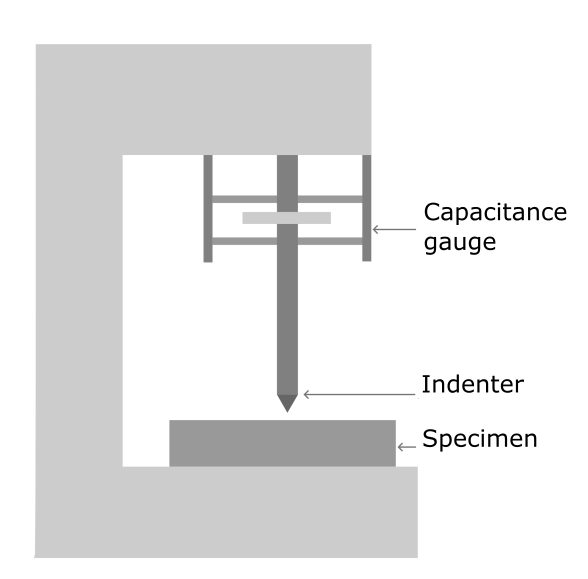
\includegraphics[width=8cm]{Images/nanoindentationbigletter}
        \decoRule
        \caption[Nanoindentation]{Nanoindentation experiment setup.}
        \label{fig:Nanoindentation}
        \end{figure}


-identation in materials
- Identation in soft materials (organs)
- Why is identation relevant in organs
-what advantages and disadvantges does identation provides
-why is relevant for this project 

%---------------------------------------------------------------------------------
\subsection{Material Modeling of Soft Materials}
 
Relevant papers tends to use hyperelastic models to represent soft materials as the viscoelasticity 
is usually neglected. 
% why do they use hyperelastic formulas? Why is it possible to neglect the viscoelasticity
%Revisar
Material model are very relevant for the simulation model (Kauer2002).
Soft tissues are approximated as near incompressible due to their highly water content.  
%viscoelastic example
For the aspiration experiment conducted by Kauer they used the following strain energy
function based on the model of Susanne and Bathe (SusanneandBAthe1987)
%Revisar


As derivative from this formula for the uteri metrial modeling the formula used was:

%---------------------------------------------------------------------------------
\subsection{Inverse Finite Element Method for Parameter Identification}

An inverse finite element (FE) approach requires usually a certain experimental model,
 which generates certain information e. g. load-displacement curve, and through 
a verified computational model match the given data curve to obtain further information 
of the material's behavior e. g., stress-strain curve.

Specially for nonlinear cases \cite{Husain2004}, where the complexity of the problems 
increases, and the interest is focused to generate an action which results in a 
certain output response, is where an inverse finite element approach can be helpful 
to discover a certain variable going from an ouput data. Through an iterative process it is 
possible to describe the material's behavior and validate the output data it 
through other established testing e. g., uniaxial testing.

Though this approach does not always give a hundred percent match in all obtain points 
or zones, it allows the researcher to understand the influences of certain parameters 
for the materials. This is specially useful for complex materials as biomaterials. 

Biomaterials, as mentioned previously, depends on multiple external factors, e.g., blood 
pressure, affected diseases and the their material properties is constantly changing. 
This issue does not allow the researcher to develop a proper material model which is 
usable for multiple use-cases. 

Therefore, the importance of the inverse element method as relevant key for estimating 
constantly changing parameters in soft materials.

For biomechanical models, where the models require knowledge from local properties \cite{Chai2013},
as the biomaterial is not isotropic; it is possible to identify a parameter e.g. Young's Modulus 
from a 3D model. The model can be matched to multiple experiments and multiple samples in different areas,
which allows a better representation of the material for further analysis.

The inverse FE approach can used by optimizing the searched parameter by matching the simulated data
to a section of a experimental curve and extending this process through some iterations. 
Nevertheless, it is important to clarify that this method also requires making assumptions to some values.
Furthermore, it is relevant to document these assumptions for the further analysis. 
With the combination of assumptions, experimental data, and a optimized and matched simulation curve, it
is possible to solve the complexity of biomechanical models.
 
In next sections some of the experimental models and the material models for bio and soft materials are 
going to be explained to get a further understanding in how is possible to get a realiable computational 
model for further reasearch

\subsubsection*{Synthetic Soft Materials}

Synthetics materials are commonly used to validate an inverse parameter identification process. 
Usually these synthetic, soft materials provide similar mechanical behavior to it's biomaterials 
counterparts. This characterization allows to validate a proposed inverse finite element approach process
before its applicatoin with a biomaterial, where the measurements to gather the experimental data are 
some in-vivo, and more challenging to recreate.


For example, Silgel, a very soft gel-like material \cite{Kauer2002} was used for the experimental 
validation of the inverse finite element method proposed, to characterized the tissue of 
a human uteri. In this work, the tensile behavior of the material was predicted through the 
parameters obtained in the aspiration method. The matching procedure is optimize through 
an objective function, which consists of the squared differences between the simulation 
and exprimental data. With an optimization algorithm an optimal set of the following parameters 
was found: the material parameters \(\mu_i\) [N/m\textsuperscript{2}] and the bulk Modulus
\(\kappa\) [N/m\textsuperscript{2}]. This method showed good prediction quality of the mentioned 
material parameters.

\subsubsection*{Biomaterials}
Biomaterials as mentioned before, represent a challenge due its difficult access and lesser replicability.
Therefore these materials are usually used for the experimetnal validation of a methd applied previously in 
synthetic materials. 
 Following the first example of the Silgel in the previous section, the inverse finite element parameter
 estimation is applied now on human uteri \cite{Kauer2002} through in vivo and ex vivo measurements of the human tissue of 
 different patients. It was mentioned, that in comparison from the silgel the uterus possesses a complex 
 multi layered structure with strongly anistropic and viscoelastic properties. Nevertheless, five 
 material parameters were determined, based on the strain energy function to model a human uterus (Yamada 1970).
Through the same inverse method applied with the synthetic material, the obtained parameters facilitated the prediction of stress-elongation curves for tensile experiments. The 
 resulting curves showed the difference of stiffness for in vivo and ex vivo measurements and the material 
 singurality for each uterus.


\subsection{Standard Verification and Validation for Computational Solid Mechanics (ASME)}
\subsubsection*{VV40}


%---------------------------------------------------------------------------------

\section{Overview}